\documentclass[11pt]{beamer}
%Gummi|065|=)

% For url referencing
\usepackage{url}
\usepackage{hyperref}

% For tables
% Create tables
\usepackage{tabularx}

% For drawing pie charts
\usepackage{pkgs/pgf-pie}

% For Creating Boxes
\usepackage{tcolorbox}

% For Algorithms
\usepackage{pkgs/algorithm2e}

% For Source Code
\usepackage{listings}
\lstset{language=python,
        numbers=left,
        numberstyle=\tiny,
        showstringspaces=false,
        aboveskip=-40pt,
        frame=leftline
        }

% For subcaptions     
\usepackage{subcaption}

% For emojis
\usepackage{tikzsymbols}

% For creating boxes
\usepackage{tcolorbox}

% For drawing flowcharts
\usepackage{tikz}
\usetikzlibrary{shapes,arrows}
% Define block styles
\tikzstyle{decision} = [diamond, draw, fill=blue!20, 
    text width=4.5em, text badly centered, node distance=3cm, inner sep=0pt]
\tikzstyle{block} = [rectangle, draw, fill=blue!20, 
    text width=5em, text centered, rounded corners, minimum height=4em]
\tikzstyle{line} = [draw, -latex']
\tikzstyle{cloud} = [draw, ellipse,fill=red!20, node distance=3cm,
    minimum height=2em]
\tikzstyle{cic} = [draw, circle,fill=red!20, node distance=3cm,
    minimum height=2em]
\tikzstyle{cic_ob} = [draw, circle,fill=red!100, node distance=3cm,
    minimum height=2em] 
    
% For inline images
\usepackage{float}   

% For Logos
\logo{%
  \makebox[0.98\paperwidth]{%
    
\includegraphics[width=3cm,keepaspectratio]{images/nrec.jpg}%
    \hfill%
    
\includegraphics[width=.7cm,keepaspectratio]{images/logo.eps}%
  }%
}
     
% Title Page        
\title{\textbf{Template for Presentation}}
\author[*]{Bikramjot Singh Hanzra \inst{}} 
\institute{ \inst{1}
		Graduate Student, 
		The Robotics Institute, 
		School of Computer Science,
		Carnegie Mellon University \\
		e-mail -- \href{mailto:bhanzra@andrew.cmu.edu}{\url{bhanzra@andrew.cmu.edu}} \\
		Homepage -- \url{andrew.cmu.edu/user/bhanzra} \\
		Blog -- \url{hanzratech.in}
		}

% YouTube Video
\usepackage{media9}  

\date{\today}

\beamertemplatenavigationsymbolsempty

\usepackage{graphicx}
\begin{document}

\begin{frame}
\maketitle
\end{frame}

% New Frame starts here
\begin{frame}
\frametitle{Enter title here}
\framesubtitle{Enter subtitle here}

Enter the content here.

To itemize use this syntax --

\begin{itemize}
\item Enter item number 1 here.
\item Enter item number 2 here.
\item Enter item number 3 here.
\end{itemize}

\end{frame}

% New Frame starts here
\begin{frame}
\label{inline-comment}
\frametitle{Enter title here}
\framesubtitle{Enter subtitle here}

To perform inline syntax highlightening in \LaTeX use, \texttt{\textbackslash texttt}, as shown below. \\

Import the OpenCV library using the command \texttt{import cv2}.

\end{frame}

% New Frame starts here
% Important -- ‘fragile’ option into the \begin{frame} command.
\begin{frame}[fragile]
\frametitle{Enter title here}
\framesubtitle{Enter subtitle here}

Code blocks can be added as shown below -- 

% REF -- http://inspirated.com/2010/03/08/using-overlays-for-source-code-listings-in-latex-beamer

\begin{semiverbatim}


\begin{lstlisting}
# Import the OpenCV Bindings
import cv2

# Load the image
im = cv2.imread('lena.png')

# Display the image
cv2.imshow("Lena Image", im)
\end{lstlisting}
\end{semiverbatim}

\end{frame}

% New Frame starts here
\begin{frame}
\frametitle{Enter title here}
\framesubtitle{Enter subtitle here}

Blocks can be added as shown below --

\begin{block}{Block Title}
This is block content.
\end{block}
Because I am using the bare design, the block does not have borders. Other designs, will have borders around the block.
\end{frame}

% New Frame starts here
\begin{frame}
\frametitle{Enter title here}
\framesubtitle{Enter subtitle here}

Blocks can be added as shown below --

\begin{block}{Block Title}
This is block content.
\end{block}
Because I am using the bare design, the block does not have borders. Other designs, will have borders around the block. \\

\textbf{Hyperref --}
\hyperlink{inline-comment}{\beamerbutton{Go to inline comments frame.}}

\end{frame}

% New Frame starts here
\begin{frame}
\frametitle{Enter title here}
\framesubtitle{Enter subtitle here}

\textbf{Pie Charts} \\

Pie charts can be added as shown in Figure \ref{pie-chart} below --

\begin{figure}[ht!]
\centering
\begin{tikzpicture}[scale=0.7]
\pie{8.57/Soccer, 57.14/Robotics, 34.29/Sleep}
\end{tikzpicture}
\caption{How I spend my day?}
\label{pie-chart}
\end{figure}

\end{frame}

% New Frame starts here
\begin{frame}
\frametitle{Enter title here}
\framesubtitle{Enter subtitle here}

\textbf{TCOLORBOX} \\

Color boxes can be added as shown below --

\begin{tcolorbox}[colback=red!5,colframe=blue!40!black,title=Put the title here]
Put the content here
\end{tcolorbox}

\end{frame}

% New Frame starts here
\begin{frame}
\frametitle{Enter title here}
\framesubtitle{Enter subtitle here}

\textbf{Algorithm} \\

\begin{algorithm}[H]
\SetAlgoLined
\KwResult{Write here the result }
 initialization\;
 \While{While condition}{
  instructions\;
  \eIf{condition}{
   instructions1\;
   instructions2\;
   }{
   instructions3\;
  }
 }
 \caption{How to write algorithms}
\end{algorithm}

\end{frame}

% New Frame starts here
\begin{frame}
\frametitle{Enter title here}
\framesubtitle{Enter subtitle here}

\textbf{FlowCharts} \\

\begin{figure}[ht!]
\centering
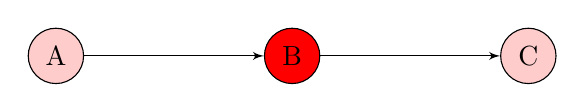
\begin{tikzpicture}[node distance = 3cm, auto]
    % Place nodes
	    \node [cic] (A) {A};
	    \node [cic_ob, right of = A] (B) {B};
	    \node [cic, right of = B] (C) {C};
    % Draw edges
    	\path [line] (A) -- (B);
    	\path [line] (B) -- (C);   	
\end{tikzpicture}
\caption{Flowchart of something in ML :)}
\label{pie-chart}
\end{figure}

\begin{figure}[ht!]
\centering
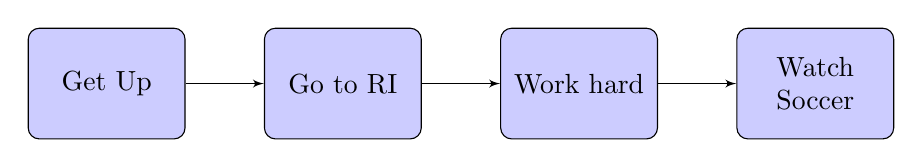
\begin{tikzpicture}[node distance = 3cm, auto]
    % Place nodes
	    \node [block] (root1) {Get Up};
    \node [block, right of=root1] (root2) {Go to RI};
    \node [block, right of=root2] (root3) {Work hard};
    \node [block, right of=root3] (root4) {Watch Soccer};
    % Draw edges
    \path [line] (root1) -- (root2);
    \path [line] (root2) -- (root3);
    \path [line] (root3) -- (root4);
\end{tikzpicture}
\caption{Flowchart of the my day}
\label{flowchart}
\end{figure}

\end{frame}

% New Frame starts here
\begin{frame}
\frametitle{Enter title here}
\framesubtitle{Enter subtitle here}

\textbf{Subfigure} \\

\begin{figure}[t!]
    \centering
    \begin{subfigure}[t]{0.5\textwidth}
        \centering
        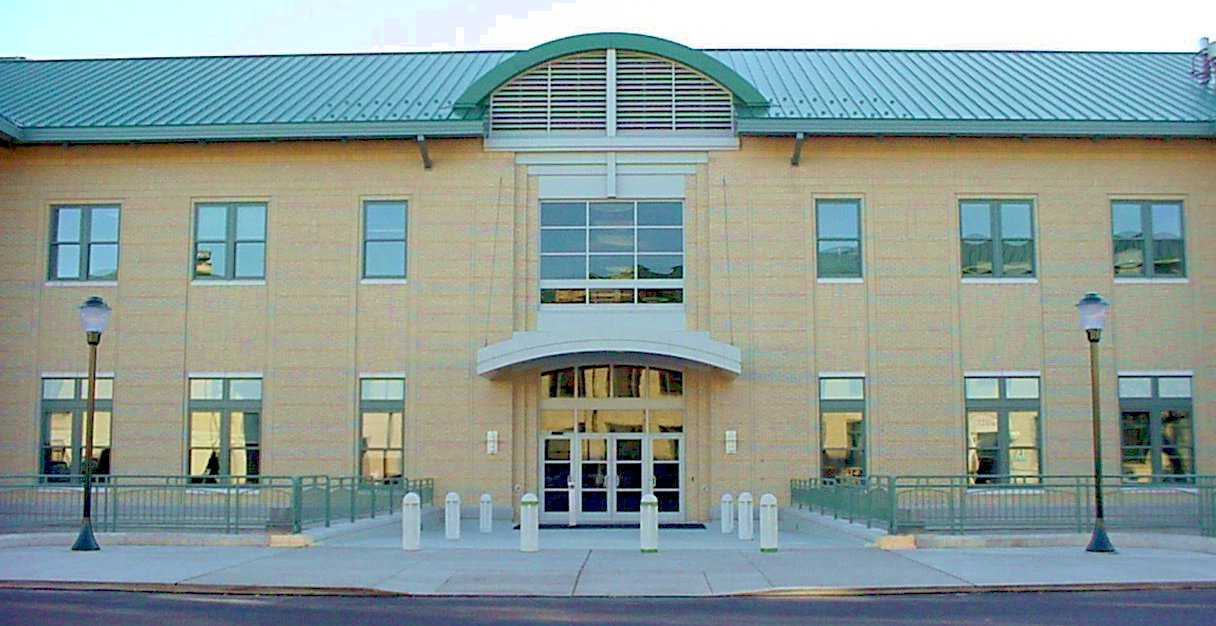
\includegraphics[scale=.1]{images/nsh.jpg}
        \caption{NSH}
        \label{caption1}
    \end{subfigure}%
    ~
    \begin{subfigure}[t]{0.5\textwidth}
        \centering
        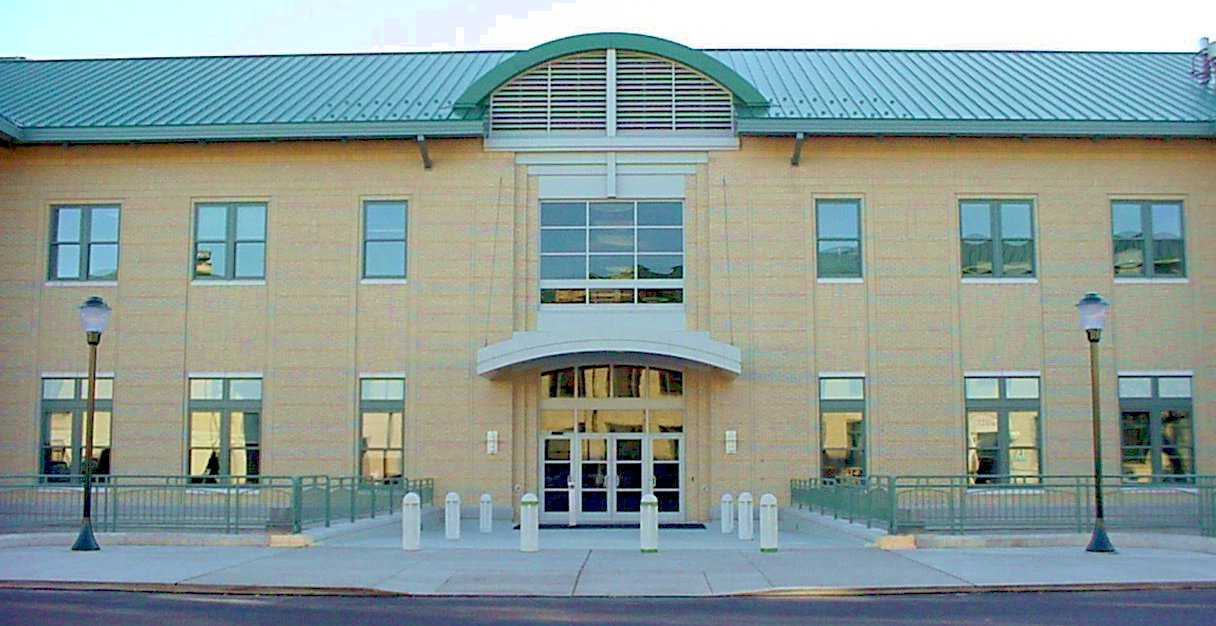
\includegraphics[scale=.1]{images/nsh.jpg}
        \caption{NSH}
        \label{caption2}
    \end{subfigure}%
    
    \centering
    \begin{subfigure}[t]{0.5\textwidth}
        \centering
        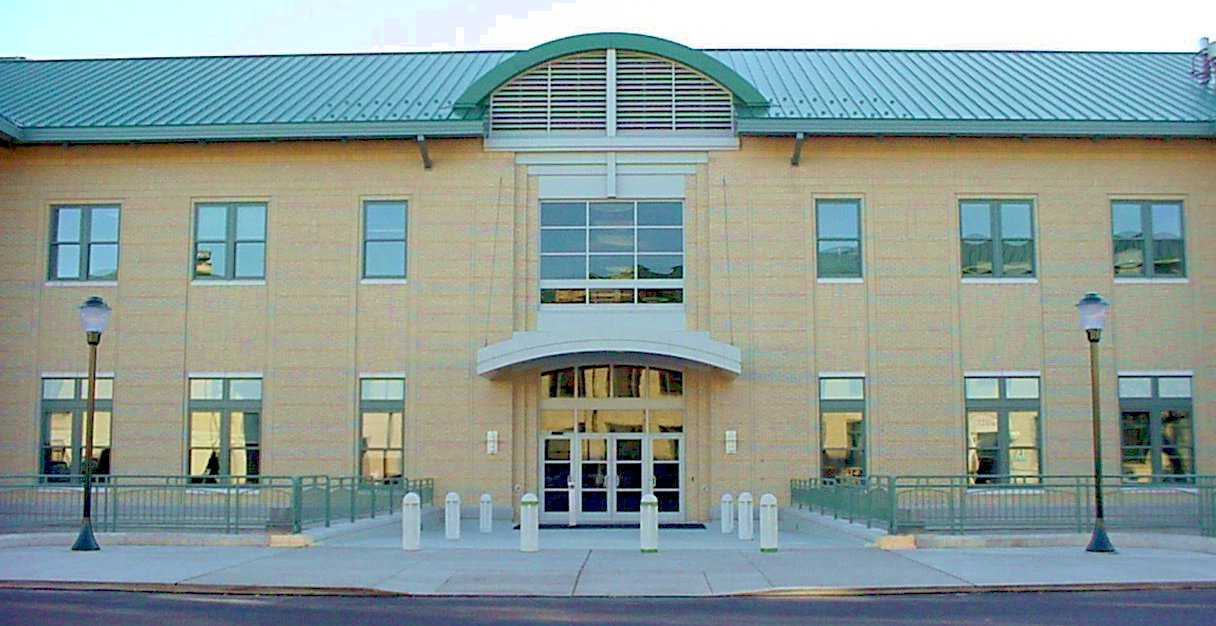
\includegraphics[scale=.1]{images/nsh.jpg}
        \caption{NSH}
        \label{caption3}
    \end{subfigure}%
    ~
    \begin{subfigure}[t]{0.5\textwidth}
        \centering
        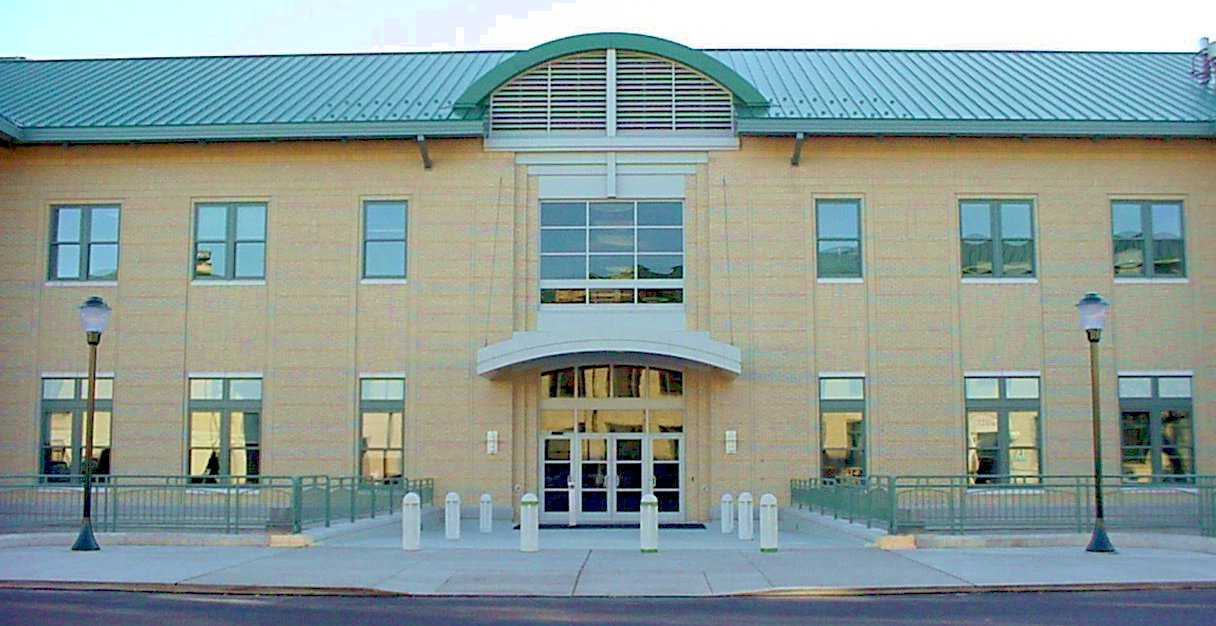
\includegraphics[scale=.1]{images/nsh.jpg}
        \caption{NSH}
        \label{caption4}
    \end{subfigure}%
    
    \caption{Subfigure Example}  
    \label{subfigure} 
\end{figure}

\end{frame}

% New Frame starts here
\begin{frame}
\frametitle{Enter title here}
\framesubtitle{Enter subtitle here}

\textbf{Tables} \\

\begin{table}[h]
\caption{Classes in $2^{nd}$ semester}
\label{ingre}

\begin{tabularx}{\textwidth}{|l|X|X|X|X|}
\hline
\textbf{Semester} & \textbf{Subject} & \textbf{Class Timings} & \textbf{Instructor}\\
\hline
$2^{nd}$ & Computer Vision & N.A. & N.A.\\
\hline
$2^{nd}$ & Mobile Robots & N.A. & N.A.\\
\hline
$2^{nd}$ & Robot Autonomy & N.A. & N.A.\\
\hline
\end{tabularx}
\end{table}

\end{frame}

% New Frame starts here
\begin{frame}
\frametitle{Enter title here}
\framesubtitle{Enter subtitle here}

\begin{columns}[c] % the "c" option specifies center vertical alignment
\column{.5\textwidth} % column designated by a command
\textbf{Columns} \\
The image on the right is of NSH, located in CMU. It is where I study !!
\column{.5\textwidth}
\begin{figure}[htp]
\centering
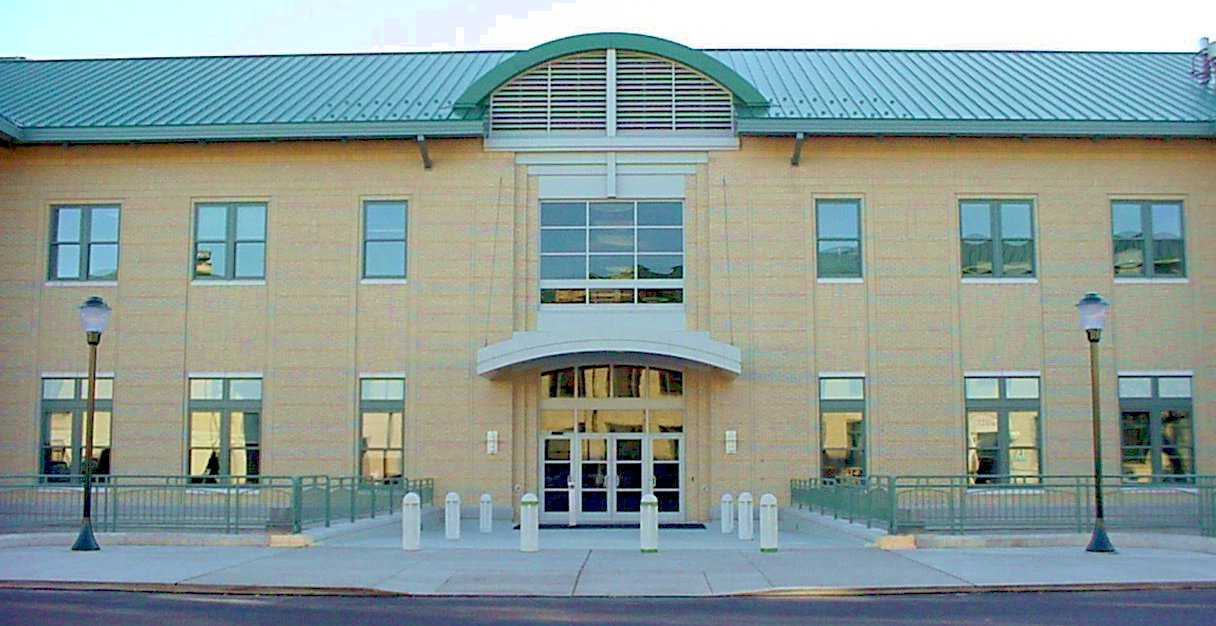
\includegraphics[scale=.1]{images/nsh.jpg}
\caption{NSH}
\label{}
\end{figure}
\end{columns}

\end{frame}

% New Frame starts here
\begin{frame}
\frametitle{Enter title here}
\framesubtitle{Enter subtitle here}

\textbf{Emojis} \\
% REF -- http://mirror.unl.edu/ctan/graphics/pgf/contrib/tikzsymbols/tikzsymbols.pdf

\dSmiley[5] 
\dSadey[5]
\dLaughey[5]
\dAnnoey[5]
\dNeutrey[5]
\dWinkey[5]
\olddWinkey[5]
\dSey[5]
\dXey[5]
\dInnocey[5]
\dCooley[5]
\dTongey[5]
\dNursey[5]
\dVomey[5]
\dWalley[5]
\drWalley[5]
\dNinja[5]



\end{frame}

% New Frame starts here
\begin{frame}
\frametitle{Enter title here}
\framesubtitle{Enter subtitle here}

\textbf{Video} \\
% REF -- http://mirror.unl.edu/ctan/graphics/pgf/contrib/tikzsymbols/tikzsymbols.pdf
\includemedia[
  width=0.6\linewidth,height=0.45\linewidth,
  activate=pageopen,
  flashvars={
    modestbranding=1 % no YT logo in control bar
   &autohide=1       % controlbar autohide
   &showinfo=0       % no title and other info before start
  }
]{}{http://www.youtube.com/v/haqjWXJOHH0?rel=0}   % Flash file
\end{frame}

\end{document}
